% Options for packages loaded elsewhere
\PassOptionsToPackage{unicode}{hyperref}
\PassOptionsToPackage{hyphens}{url}
\PassOptionsToPackage{dvipsnames,svgnames,x11names}{xcolor}
%
\documentclass[
  11pt,
  letterpaper,
  DIV=11,
  numbers=noendperiod]{scrartcl}

\usepackage{amsmath,amssymb}
\usepackage{iftex}
\ifPDFTeX
  \usepackage[T1]{fontenc}
  \usepackage[utf8]{inputenc}
  \usepackage{textcomp} % provide euro and other symbols
\else % if luatex or xetex
  \usepackage{unicode-math}
  \defaultfontfeatures{Scale=MatchLowercase}
  \defaultfontfeatures[\rmfamily]{Ligatures=TeX,Scale=1}
\fi
\usepackage{lmodern}
\ifPDFTeX\else  
    % xetex/luatex font selection
\fi
% Use upquote if available, for straight quotes in verbatim environments
\IfFileExists{upquote.sty}{\usepackage{upquote}}{}
\IfFileExists{microtype.sty}{% use microtype if available
  \usepackage[]{microtype}
  \UseMicrotypeSet[protrusion]{basicmath} % disable protrusion for tt fonts
}{}
\makeatletter
\@ifundefined{KOMAClassName}{% if non-KOMA class
  \IfFileExists{parskip.sty}{%
    \usepackage{parskip}
  }{% else
    \setlength{\parindent}{0pt}
    \setlength{\parskip}{6pt plus 2pt minus 1pt}}
}{% if KOMA class
  \KOMAoptions{parskip=half}}
\makeatother
\usepackage{xcolor}
\setlength{\emergencystretch}{3em} % prevent overfull lines
\setcounter{secnumdepth}{5}
% Make \paragraph and \subparagraph free-standing
\makeatletter
\ifx\paragraph\undefined\else
  \let\oldparagraph\paragraph
  \renewcommand{\paragraph}{
    \@ifstar
      \xxxParagraphStar
      \xxxParagraphNoStar
  }
  \newcommand{\xxxParagraphStar}[1]{\oldparagraph*{#1}\mbox{}}
  \newcommand{\xxxParagraphNoStar}[1]{\oldparagraph{#1}\mbox{}}
\fi
\ifx\subparagraph\undefined\else
  \let\oldsubparagraph\subparagraph
  \renewcommand{\subparagraph}{
    \@ifstar
      \xxxSubParagraphStar
      \xxxSubParagraphNoStar
  }
  \newcommand{\xxxSubParagraphStar}[1]{\oldsubparagraph*{#1}\mbox{}}
  \newcommand{\xxxSubParagraphNoStar}[1]{\oldsubparagraph{#1}\mbox{}}
\fi
\makeatother


\providecommand{\tightlist}{%
  \setlength{\itemsep}{0pt}\setlength{\parskip}{0pt}}\usepackage{longtable,booktabs,array}
\usepackage{calc} % for calculating minipage widths
% Correct order of tables after \paragraph or \subparagraph
\usepackage{etoolbox}
\makeatletter
\patchcmd\longtable{\par}{\if@noskipsec\mbox{}\fi\par}{}{}
\makeatother
% Allow footnotes in longtable head/foot
\IfFileExists{footnotehyper.sty}{\usepackage{footnotehyper}}{\usepackage{footnote}}
\makesavenoteenv{longtable}
\usepackage{graphicx}
\makeatletter
\def\maxwidth{\ifdim\Gin@nat@width>\linewidth\linewidth\else\Gin@nat@width\fi}
\def\maxheight{\ifdim\Gin@nat@height>\textheight\textheight\else\Gin@nat@height\fi}
\makeatother
% Scale images if necessary, so that they will not overflow the page
% margins by default, and it is still possible to overwrite the defaults
% using explicit options in \includegraphics[width, height, ...]{}
\setkeys{Gin}{width=\maxwidth,height=\maxheight,keepaspectratio}
% Set default figure placement to htbp
\makeatletter
\def\fps@figure{htbp}
\makeatother

% styles.tex
%\usepackage{cmbright}
\usepackage[dvipsnames]{xcolor}
\usepackage{sectsty}
\usepackage{titlesec}
\usepackage{tikz}
\usepackage{graphicx}

% Define red, centered Day headers
\titleformat{\section}
  {\normalfont\color{black}\centering\LARGE\bfseries}
  {\thesection}{1em}{}

\definecolor{flashcolor}{RGB}{221,217,195}

% Optional: Adjust subsection and subsubsection if desired
% \titleformat{\subsection}
%   {\normalfont\large\bfseries}{\thesubsection}{1em}{}
\KOMAoption{captions}{tableheading}
\makeatletter
\@ifpackageloaded{caption}{}{\usepackage{caption}}
\AtBeginDocument{%
\ifdefined\contentsname
  \renewcommand*\contentsname{Table of contents}
\else
  \newcommand\contentsname{Table of contents}
\fi
\ifdefined\listfigurename
  \renewcommand*\listfigurename{List of Figures}
\else
  \newcommand\listfigurename{List of Figures}
\fi
\ifdefined\listtablename
  \renewcommand*\listtablename{List of Tables}
\else
  \newcommand\listtablename{List of Tables}
\fi
\ifdefined\figurename
  \renewcommand*\figurename{Figure}
\else
  \newcommand\figurename{Figure}
\fi
\ifdefined\tablename
  \renewcommand*\tablename{Table}
\else
  \newcommand\tablename{Table}
\fi
}
\@ifpackageloaded{float}{}{\usepackage{float}}
\floatstyle{ruled}
\@ifundefined{c@chapter}{\newfloat{codelisting}{h}{lop}}{\newfloat{codelisting}{h}{lop}[chapter]}
\floatname{codelisting}{Listing}
\newcommand*\listoflistings{\listof{codelisting}{List of Listings}}
\makeatother
\makeatletter
\makeatother
\makeatletter
\@ifpackageloaded{caption}{}{\usepackage{caption}}
\@ifpackageloaded{subcaption}{}{\usepackage{subcaption}}
\makeatother

\ifLuaTeX
  \usepackage{selnolig}  % disable illegal ligatures
\fi
\usepackage{bookmark}

\IfFileExists{xurl.sty}{\usepackage{xurl}}{} % add URL line breaks if available
\urlstyle{same} % disable monospaced font for URLs
\hypersetup{
  colorlinks=true,
  linkcolor={blue},
  filecolor={Maroon},
  citecolor={Blue},
  urlcolor={Blue},
  pdfcreator={LaTeX via pandoc}}


\author{}
\date{}

\begin{document}

\begin{titlepage}
\centering


\includegraphics[width=0.8\textwidth]{UofGMS_header.png}

\vspace*{4cm}

\noindent\rule{\textwidth}{1pt}
{\Huge \bfseries Challenges in environmental spatio-temporal modelling \par}

{\Large \bfseries Part of the EPSRC-funded project GEOBEx\par}

{\large \bfseries 16 June 2025 University of Glasgow, UK\par}

\noindent\rule{\textwidth}{1pt}
\vspace{1.5cm}

%{\fontsize{30}{28}\selectfont \bfseries Book of abstracts\par}
%\vspace{1.5cm}

%\includegraphics[width=0.3\textwidth]{hr_pic.png}

\begin{tikzpicture}[remember picture,overlay]
  \node[anchor=south west,inner sep=0pt]
       at ([xshift=30mm,yshift=10mm]current page.south west)
       {
\includegraphics[width=0.7\textwidth]{UofGMS_footer.png}};
\end{tikzpicture}

%\begin{tikzpicture}[remember picture,overlay]
%  \coordinate (anchor) at ([xshift=150mm,yshift=200mm]current page.south west);
%  \node[anchor=south west,inner sep=0pt] at (current page.south west)
%       {
\includegraphics[width=0.7\textwidth]{UofGMS_footer.png}};
%\end{tikzpicture}

%\begin{picture}(0,0)
%  \put(0,0){
\includegraphics[width=0.6\textwidth]{UofGMS_footer.png}}
%\end{picture}

\end{titlepage}
\clearpage
\setcounter{page}{1}

\renewcommand*\contentsname{Table of contents}
{
\hypersetup{linkcolor=}
\setcounter{tocdepth}{3}
\tableofcontents
}

\newpage

\section{About the workshop}\label{about-the-workshop}

This one-day workshop marks the conclusion of the EPSRC-funded project
GEOBEx: Geostatistics Binary Models for Extremes, led by Carolina Euan
(Lancaster University) and Daniela Castro-Camilo (University of
Glasgow). The project has focused on the development of novel
methodologies for modelling spatial binary extremes, with applications
to environmental problems. It serves as a compelling illustration of
areas in spatio-temporal environmental statistics that require further
development, providing valuable insights into current challenges and
potential solutions.

The workshop aims to bring together a small group of researchers with
shared interests in spatio-temporal environmental statistics and the
environmental sciences more broadly. It offers a space for open,
collaborative discussion and the exchange of ideas across disciplines
and career stages.

\textbf{Goals}

\begin{itemize}
\item
  Facilitate dialogue on challenges and opportunities in modelling
  spatial and spatio-temporal environmental extremes.
\item
  Encourage collaboration by bringing together researchers from academia
  and applied fields.
\item
  Identify future directions for methodological and applied development.
\item
  Foster knowledge exchange, with participants sharing a one-slide
  summary of their work and selected 15-minute talks on current research
  related to environmental problems.
\end{itemize}

We hope that this collective effort will pave the way for stronger
interdisciplinary connections and more impactful applications of
environmental statistics.

\newpage

\section{Location}\label{location}

We will meet in Seminar Room 311B, located on the third floor of the
Mathematics and Statistics Building
(\href{https://www.google.com/maps/place/School+of+Mathematics+and+Statistics/@55.8726073,-4.2944843,871m/data=!3m2!1e3!4b1!4m6!3m5!1s0x488845cfd066d839:0xeab86bed8f92f0d0!8m2!3d55.8726073!4d-4.2944843!16s\%2Fg\%2F11ddzkn8v0?entry=ttu&g_ep=EgoyMDI1MDYwMS4wIKXMDSoASAFQAw\%3D\%3D}{Google
map}). The room is accessible by both stairs and lift. The building is
just a 6-minute walk from Hillhead subway station.

\begin{center}
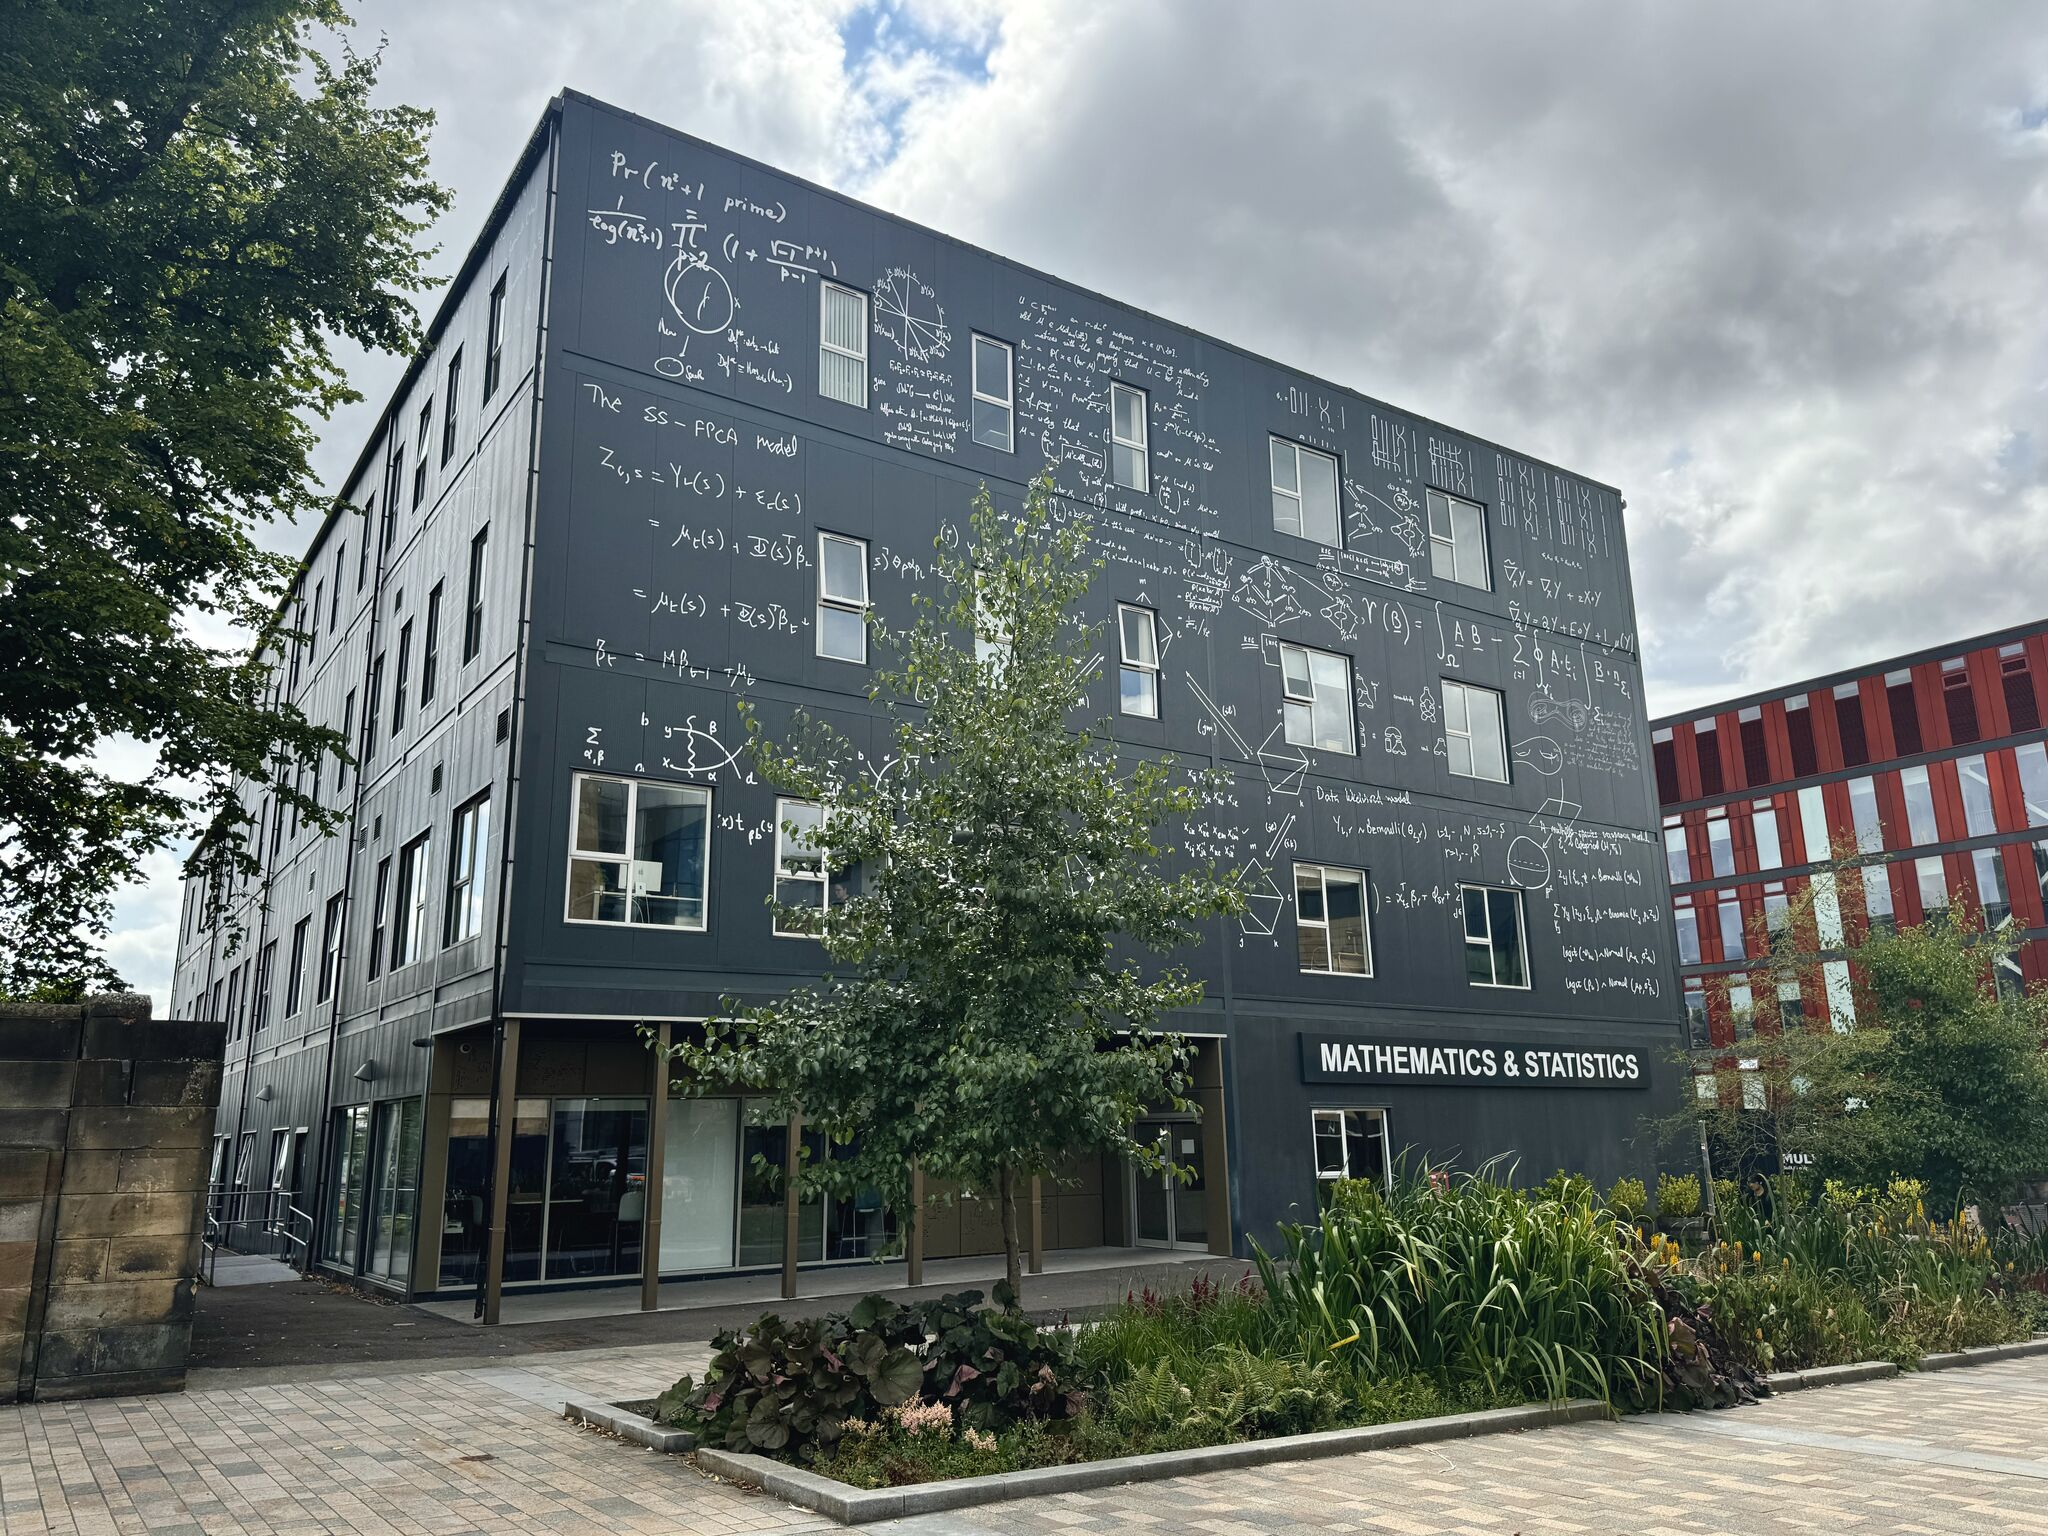
\includegraphics[width=0.6\linewidth]{ms-building.jpg}
\end{center}

\begin{center}
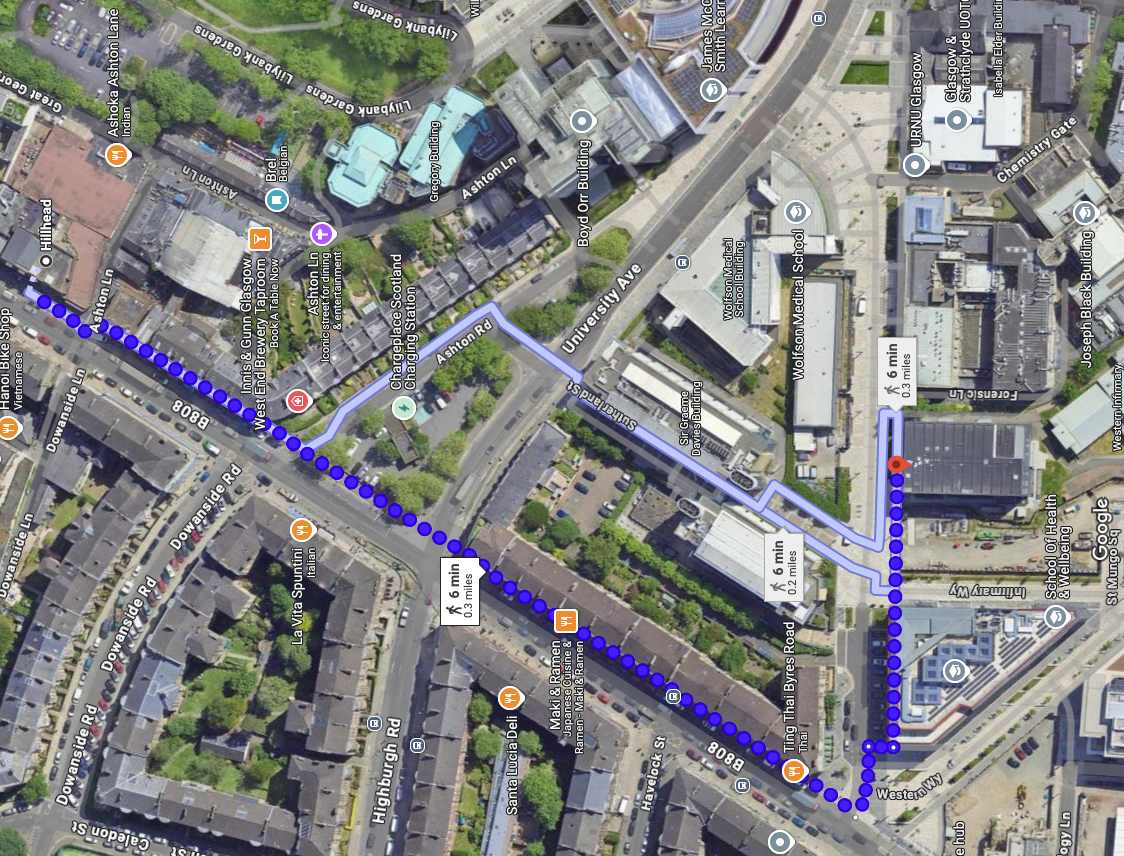
\includegraphics[width=0.6\linewidth]{map-to-ms.png}
\end{center}

\newpage

\section{Programme overview}\label{programme-overview}

\textbf{10:00-10:20} --- Opening and summary of the GEOBEx project

\textbf{10:20-10:50} --- 3-minute introductions from each participant

\textbf{10:50-11:20} --- Coffee break

\textbf{11:20-12:20 --- Morning Talks}

\begin{itemize}
\item
  \textbf{11:20-11:35} --- Marian Scott (University of Glasgow):
  \emph{Environmental digital twins --- challenges and opportunities}
\item
  \textbf{11:35-11:50} --- Claire Miller (University of Glasgow):
  \emph{Challenges in spatiotemporal modelling of national scale river
  water catchments}
\item
  \textbf{11:50-12:05} --- Claire Risley (EA): \emph{Current Challenges
  for the Environment Agency in Spatial Statistics}
\item
  \textbf{12:05-12:20} --- Ben Marchant (BGS): \emph{Space-time
  challenges at the British Geological Survey}
\end{itemize}

\textbf{12:20-13:30} --- Lunch

\textbf{13:30-14:30 --- Afternoon Talks}

\begin{itemize}
\item
  \textbf{13:30-13:45} --- Israel Martínez-Hernández (Lancaster
  University): \emph{Modelling large spatio-temporal data: A short,
  medium, and long term wind forecast}
\item
  \textbf{13:45-14:00} --- Dave Miller (BioSS): \emph{Adding structure
  to regression-like ecological models}
\item
  \textbf{14:00-14:15} --- Michael Tso (UKCEH): \emph{Adaptive sampling
  for high-frequency nutrient sensors}
\item
  \textbf{14:15-14:30} --- Craig Wilkie (University of Glasgow):
  \emph{Data fusion approaches for environmental data}
\end{itemize}

\textbf{14:30-15:00} --- Coffee break

\textbf{15:00-16:30} --- Group discussion

\textbf{17:30-19:45} --- Dinner at
\href{https://bothyglasgow.co.uk/}{The Bothy}, 11 Ruthven Ln, Glasgow,
G12 9BG
\href{https://www.google.com/maps/dir/Mathematics+and+Statistics+Building,+132+University+Pl,+Glasgow+G12+8TA,+UK/Bothy+Glasgow,+Ruthven+Lane,+Glasgow/@55.8739913,-4.2977924,511m/data=!3m2!1e3!4b1!4m14!4m13!1m5!1m1!1s0x488845cfd066d839:0xeab86bed8f92f0d0!2m2!1d-4.2944843!2d55.8726073!1m5!1m1!1s0x488845cf1ccbb223:0x8ef11cd374daaf1d!2m2!1d-4.2944528!2d55.8753694!3e3?entry=ttu&g_ep=EgoyMDI1MDYwNC4wIKXMDSoASAFQAw\%3D\%3D}{(click
here for directions from The Maths \& Stats Building)}

\newpage

\section{Abstracts}\label{abstracts}

The grouping and sequence of talks aim to gradually build context---from
general frameworks and national challenges to specific methods and
applications---while maintaining variety and thematic coherence.

\subsection{Opening / Framing the
Landscape}\label{opening-framing-the-landscape}

\subsubsection[\textbf{Marian Scott} (University of Glasgow) \\Environmental digital twins — challenges and opportunities]{Marian Scott (University of Glasgow)}

\textbf{Title}: Environmental digital twins --- challenges and
opportunities

\textbf{Summary.} Increasingly more and more data are being generated on
environmental systems, from new sensors and also earth observation
missions. However the governance of such data sources is fragmented, and
the first challenge we have is in discovering and linking these
disparate data sources. At the same time, there are a number of
integrative models, offering holistic views of the ``system''. It is in
this context that digital twins are being developed. They offer a
dynamic system view, informed/learning from data, they are a digital
replica of the environmental system and there is a bi-directional flow
of intelligence from real-virtual and virtual- real. Their main power
lies in their predictive capacity, and the testing of different future
scenarios. In this short presentation, I will focus on water and present
a framework for catchment (river basin) modelling of water quality and
quantity.

\subsection{National-Scale Environmental Monitoring
Challenges}\label{national-scale-environmental-monitoring-challenges}

\subsubsection[\textbf{Claire Miller} (University of Glasgow) \\Challenges in spatiotemporal modelling of national scale river water catchments]{Claire Miller (University of Glasgow)}

\textbf{Title}: Challenges in spatiotemporal modelling of national scale
river water catchments

\textbf{Summary.} In recent years, with an increasing number of emerging
potential contaminants, the potential combined effect of multiple
chemicals on river water quality has become of greater interest.
Additionally, there are knowledge gaps around the effects of
hydrological, climate and landscape changes, in combination with
different mixtures of chemicals, on freshwater species in river water
catchments. This presentation will introduce the related statistical and
data analytics challenges and developments being explored through
projects such as NERC MOT4Rivers.

\subsubsection[\textbf{Claire Risley} (Environmental Agency) \\Current Challenges for the Environment Agency in Spatial Statistics]{Claire Risley (Environmental Agency)}

\textbf{Title}: Current Challenges for the Environment Agency in Spatial
Statistics

\textbf{Summary.} Claire will showcase spatial statistics projects she
has contributed to during her time at the EA.

\subsection{Institutional Perspectives on Spatio-Temporal
Modelling}\label{institutional-perspectives-on-spatio-temporal-modelling}

\subsubsection[\textbf{Ben Marchant} (BGS) \\Space-time challenges at the British Geological Survey]{Ben Marchant (BGS)}

\textbf{Title}: Space-time challenges at the British Geological Survey

\textbf{Summary.} Scientists at the British Geological Survey study many
earth science systems that vary in space and time. These include the
variation of groundwater levels and quality, the occurrence of
landslides, vertical ground motion, the temperature of subsurface water
that can provide geothermal heating and space-weather which can impact
communication systems. There is often a need to make spatial and
temporal predictions of key properties of these systems and to test
hypotheses regarding the main drivers of variation. However, such
analyses can be hampered by the complexity and heterogeneity of the
systems, the number of measurements to be analysed and the use of legacy
data where sampling locations may have been selected purposively. I will
illustrate these points with reference to BGS work on the variation of
groundwater levels and more generally discuss our remaining space-time
challenges.

\subsection{Statistical Methods for Complex Spatio-Temporal
Data}\label{statistical-methods-for-complex-spatio-temporal-data}

\subsubsection[\textbf{Israel Martínez-Hernández} (University of Lancaster) \\Modelling large spatio-temporal data: A short, medium, and long term wind forecast]{
Israel Martínez-Hernández (University of Lancaster)}

\textbf{Title}: Modelling large spatio-temporal data: A short, medium,
and long term wind forecast

\textbf{Summary.} Due to the rapid development of complex, performant
technologies, spatio-temporal data can now be collected on a large
scale. However, the statistical modelling of large sets of
spatio-temporal data involves several challenging problems, particularly
regarding computational demands. I will present a new methodology to
model complex and large spatio-temporal datasets. This approach invloves
estimating a continuous surface at each time point, effectively
capturing spatial dependence, possibly nonstationary. As a result, the
spatio-temporal data can be seen as a sequence of surfaces. Then, we
model this sequence of surfaces using functional time series techniques.
The functional time series approach allows us to obtain a
computationally feasible methodology and also provides extensive
flexibility in terms of time forecasting. We illustrate these advantages
using a high-resolution wind speed simulated dataset of over 4 million
values.

\subsubsection[\textbf{Dave Miller} (BioSS) \\Adding structure to regression-like ecological models]{Dave Miller (BioSS)}

\textbf{Title}: Adding structure to regression-like ecological models

\textbf{Summary.} Covariates that occur in ecological and environmental
science are often inherently non-scalar, sometimes having a spatial or
temporal structure of their own. While aggregating or selectively
summarizing such covariates to yield a scalar covariate allows use of
standard regression models, exactly how to do so can be problematic,
e.g., using a mean or median of some subsequence of a time series. Here
I'll talk about three useful extensions that fit in the GAM framework
(varying-coefficient, scalar-on-function and distributed lag models)
that can be used to add more structure to our models and the connections
between these approaches. Although these models are a useful basic set
of tools, I'll also discuss further advances that would enhance our
modelling of highly structured data further.

Joint work with Ken Newman and Thomas Cornulier (BioSS)

\subsection{Adaptive \& Intelligent
Monitoring}\label{adaptive-intelligent-monitoring}

\subsubsection[\textbf{Michael Tso} (UKCEH) \\Adaptive sampling for high-frequency nutrient sensors ]{Michael Tso (UKCEH)}

\textbf{Title}: Adaptive sampling for high-frequency nutrient sensors

\textbf{Summary.} Traditional environmental monitoring employs fixed
designs, which do not vary over the survey duration. Adaptive sampling
uses previously collected data to inform and vary a sample design over
the course of a monitoring period to offer a more optimal and flexible
data collection. Existing work on adaptive sampling has mostly been
focused on spatial survey designs. Here we highlight the potential of
adopting adaptive sampling principles by varying frequency of
environmental sensors, which we are motivated by a new generation of
high-frequency `lab-on-a-chip' sensors. Even though these sensors
feature low reagent consumption, measuring at very high frequency
continuously comes with high energy, computational, data storage, and
analysis costs and challenges. We envisage sensors to be configured to
maintain a basic level of monitoring and record data continuously, while
only being triggered to monitor at a very high frequency when certain
data-driven conditions are met (and then return to baseline monitoring).
The datasets and criteria to inform the triggering can be highly
adaptable. For datasets, with sophistication increases, it can include
data on the sensor itself, other collocated sensors, other sensors in
the region, remote sensing data, stormwater overflow, or weather
forecasts. For criteria, it can be based on user-defined thresholds,
domain expert knowledge, or statistical methods such as changepoints,
clustering, or Bayesian adaptive sampling. We illustrate our approach
with examples and a R package. We welcome contributions to this ongoing
work, particularly in addressing stakeholder concerns, such as
robustness in statistical analysis of multi-frequency data and the
detection of extreme events.

Joint work with: Peter A Henrys, Eleanor Mackay, Xize Niu (UK Centre for
Ecology \& Hydrology and University of Southampton)

\subsection{Data Fusion and
Integration}\label{data-fusion-and-integration}

\subsubsection[\textbf{Craig Wilkie} (University of Glasgow) \\Data fusion approaches for environmental data]{Craig Wilkie (University of Glasgow)}

\textbf{Title}: Adaptive sampling for high-frequency nutrient sensors

\textbf{Summary.} Increasing availability of environmental data from
multiple sources such as satellites and low-cost sensors provides us
with improved understanding of our changing environment. However, data
from these disparate sources can be of varying quality, and often on
different spatial and temporal scales. Data fusion approaches are
designed to combine information from multiple sources to provide an
enhanced understanding of environmental variables, with associated
uncertainty measures that account for differences in the quality of the
information provided by each source. This talk will present statistical
data fusion approaches, with possible extensions to modelling extreme
values.

\newpage

\section{Proposed topics for
discussion}\label{proposed-topics-for-discussion}

Feel free to use the topics below as a guide---they're entirely
optional, so you're welcome to include others or leave them out.

\subsection{Theme 1: Data Complexity and
Integration}\label{theme-1-data-complexity-and-integration}

\textbf{Relevant talks}: Marian Scott, Claire Miller, Ben Marchant,
Craig Wilkie

\textbf{Prompt questions}:

\begin{itemize}
\item
  What are the most pressing barriers to integrating heterogeneous
  environmental data sources?
\item
  How can we balance model complexity with interpretability when fusing
  diverse datasets?
\item
  Are there good examples of success (or failure) in multi-source
  integration we can learn from?
\end{itemize}

\subsection{Theme 2: Modelling Choices and
Scalability}\label{theme-2-modelling-choices-and-scalability}

\textbf{Relevant talks}: Dave Miller, Israel Martínez-Hernández, Michael
Tso

\textbf{Prompt questions}:

\begin{itemize}
\item
  What modelling approaches scale best to large or high-frequency
  datasets?
\item
  How do we decide between simpler models (e.g., regression/GAMs) and
  complex hierarchical or functional models?
\item
  What compromises have you made between model flexibility and
  computational feasibility?
\end{itemize}

\subsection{Theme 3: Decision-Driven
Modelling}\label{theme-3-decision-driven-modelling}

\textbf{Relevant talks}: Claire Miller, Claire Risley, Michael Tso

\textbf{Prompt questions}:

\begin{itemize}
\item
  How do we make our models useful for decision-makers and
  practitioners?
\item
  What statistical uncertainties matter most in practice, and how should
  we communicate them?
\item
  How do we build adaptive systems that react to real-time information?
\end{itemize}

\subsection{Theme 4: Collaboration and
Co-Production}\label{theme-4-collaboration-and-co-production}

All talks are relevant here

\textbf{Prompt questions}:

\begin{itemize}
\item
  What has helped or hindered successful collaboration across academia,
  agencies, and industry?
\item
  What would an ideal collaborative workflow look like for tackling a
  spatio-temporal environmental problem?
\item
  Are there shared needs (e.g., open datasets, tools, training) that we
  could address together?
\end{itemize}




\end{document}
